\documentclass{article}
% =======PACKAGES=======
% FORMATTING
\usepackage[margin=0.625in]{geometry}
\usepackage{parskip, setspace}
\setstretch{1.15}
% TYPESETTING - MATH
\usepackage{amsmath, amsfonts}
\usepackage[ruled, linesnumbered, noend]{algorithm2e}
\usepackage{listings}
\usepackage{xcolor}

\lstdefinestyle{mystyle}{
    backgroundcolor=\color{lightgray},   
    commentstyle=\color{darkgray},
    keywordstyle=\color{red},
    numberstyle=\color{black},
    stringstyle=\color{violet},
    basicstyle=\ttfamily\footnotesize,
    breakatwhitespace=false,         
    breaklines=true,                 
    captionpos=b,                    
    keepspaces=true,                 
    numbers=left,                    
    numbersep=5pt,                  
    showspaces=false,                
    showstringspaces=false,
    showtabs=false,                  
    tabsize=2
}
\lstset{style=mystyle}
% RICH
\usepackage{graphicx, caption}
\usepackage{hyperref}
% BIBLIOGRAPHY
\usepackage[
backend=biber,
sorting=ynt
]{biblatex}
\addbibresource{bib.bib}

% =======TITLE=======
\title{\vspace*{-0.625in}CS 529: Advanced Data Structures \& Algorithms \\ Assignment 2: $k$-d Trees}
\author{Nathan Chapman, Hunter Lawrence, Andrew Struthers}
\date{\today}

\begin{document}

    \maketitle
    \section*{Introduction of KD Trees}
Because of the hierarchical nature of KD trees, we can organize data points with a tree structure. To construct a KD tree, we can recursively partition the dataset into subsets along different dimensional axes. At each level of the tree, a dimension is chosen to split the data, creating a node with a hyperplane representing this division. We can then repeat this process until each leaf node corresponds to a single data point.

A KD tree is efficient because of the functionality that lets us discard entire subtrees during the search process, like other tree structures do. This reduces the number of distance calculations required when performing a Nearest Neighbor Search (NNS). When querying for the nearest neighbor, we traverse the tree, comparing distances between the query point and the hyperplanes at each node. Subtrees that are farther away from the query point than the current best distance can be pruned, significantly speeding up the search.

Nearest Neighbor Search is a fundamental concept in machine learning and data analysis, where the goal is to find the data point in a dataset that is closest to a given query point. KD trees, or k-dimensional trees, are a data structure designed to efficiently perform NNS in multidimensional spaces.

\begin{figure}[h]
    \centering
    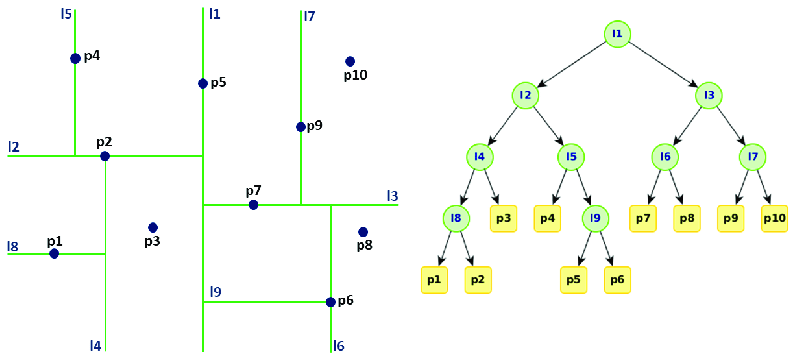
\includegraphics[width=\textwidth,keepaspectratio]{Images/space_partition.png}
    \label{fig:space_partition}
    \caption{Visualization of a KD Tree structure being used to partition points along 2 dimensional hyperplanes}
\end{figure}

KD trees find applications in various machine learning tasks. One of the more common uses is in K-nearest neighbors (KNN) algorithms, where we want to classify a data point based on the class of its nearest neighbors. KD trees enhance the performance of KNN by efficiently locating these neighbors, making the algorithm computationally feasible for large datasets.

Another application is in approximate nearest neighbor search, where we want points whose distance from the given point is some scalar multiple of the distance from the query to its nearest points. This is useful if we wanted to find all points within a certain distance of a given point, which has applications when finding clusters or finding neighborhoods of data points. KD trees can be adapted to balance exactness while still having logarithmic computational efficiency in such scenarios, which lets us have fast retrieval of similar data points.

KD trees aren't perfect for every scenario, however. Despite their advantages, KD trees usually struggle with the curse of high dimensionality, and they exhibit limitations in high-dimensional spaces. As the number of dimensions increases, the effectiveness of KD trees diminishes, and alternative methods might be better.

KD trees provide an efficient logarithmic solution for Nearest Neighbor Search in machine learning by organizing data in a hierarchical structure and pruning irrelevant subtrees during the search process. While they are very good in low-dimensional spaces, performance degradation happens in high-dimensional data.

    \section*{KD Tree Technical Information}
KD trees are a binary tree structure which stores multidimensional data with priority placed on the ability to find a nearest neighbor. These trees do not place data in perfectly sorted order, but instead cyclically compares dimensions at each layer of the tree. Consider a tree built for a three dimensional object with the dimensions $x_1$, $x_2$, $x_3$. At layer 0: $x_1$ is evaluated (anything with objectively less or more value than $x_1$ is placed into the left or right subtree), at layer 1: $x_2$ is evaluated, at layer 2: $x_3$ is evaluated, and once at layer 3: $x_1$ is evaluated again, and the cycle will continue to repeat. It is important to keep in mind that not all attributes are considered at each layer, meaning that it is possible to have $x_2$ values in layer 0’s left subtree which may be greater than values in layer 0’s right subtree. Consider the following example from John Louis Bentley’s Multidimensional Binary Search Trees In Database Applications from 1978:

\begin{figure}[h]
    \centering
    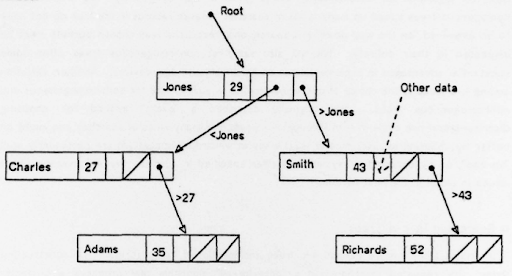
\includegraphics[width=\textwidth,keepaspectratio]{Images/kd_tree.png}
    \label{fig:kd_tree}
    \caption{Bentley, John Louis. Multidimensional Binary Search Trees in Database Applications. September 8, 1978. Department of computer science and mathematics Carnegie-Mellon University. Pittsburgh; Pennsylvania 15213. Pg. 6.}
\end{figure}


In this example, the first attribute to be evaluated was the alphabetical order of the names, then the second attribute was some number (assumed to be age). Since the first attribute was evaluated without consideration to the second, everyone in the left subtree has names with a value ``less than" ``Jones". However, it is possible for individuals in the left subtree to have an age greater than the original object ``Jones". Hence ``Adams" could make it to the left subtree of ``Jones" with the higher age of 35, as well as being placed in the right subtree of ``Charles", despite having a name with an objectively lower value. This is due to sole consideration of each dimension’s attribute within its respective layer.

K-D Tree traversal for search, insert, and delete operations are achieved in $O(\text{log} n)$ average time, and $O(n)$ worst case time. But the major strength of KD Trees lies in its ability to find the nearest neighbor in an average run time of $O(\text{log} n)$.


        \section*{Formalizing the Nearest Neighbor Search using $k$-D Trees in Machine Learning}

            We begin with the psuedo-code of the NNS, adapted from Python\cite{CMUSlides}.

            \begin{function}
                \caption{NN(Point Q, kdTree T, int cd, Rect BB)}
                \DontPrintSemicolon

                \KwIn{Point, $k$-d Tree, Integer, Rectangle}
                \KwOut{}

                \tcp{if this bounding box is too far, do nothing}
                \If{T does not exist or the distance between Q and BB is more than the current best}{
                    \Return{}
                }

                \tcp{if this point is better than the best}
                $dist \gets$ distance between $Q$ and $T.data$\;
                \If{dist $<$ distance between Q and T.data}{
                    $best \gets$ T.data\;
                    best\_distance $\gets$ dist
                }

                \tcp{visit subtrees in most promising oder}
                \eIf{Q[cd] $<$ T.data[cd]}{
                    \NN(Q, T.left, next\_cd, BB.trimLeft(cd, t.data))\;
                    \NN(Q, T.right, next\_cd, BB.trimRight(cd, t.data))
                }{
                    \NN(Q, T.right, next\_cd, BB.trimRight(cd, t.data))\;
                    \NN(Q, T.left, next\_cd, BB.trimLeft(cd, t.data))
                }
            \end{function}

            If we don't want to reinvent the machine-learning-wheel, one of the main ways to use machine learning today is to use Python's \texttt{scikit-learn} package.  There are two ways of using $k$-D-tree-based nearest neighbor searching with \texttt{scikit-learn}\cite{sklearn_api}: directly calling \texttt{NearestNeighbors} and choosing \texttt{algorithm = KDTree}, or by first building a $k$-D Tree and subsequently querying it.

            For example, directly calling \texttt{NearestNeighbors}: 

            \begin{lstlisting}[language = Python, caption = \texttt{NearestNeighbors}]
from sklearn.neighbors import NearestNeighbors
import numpy as np
X = np.array([[-1, -1], [-2, -1], [-3, -2], [1, 1], [2, 1], [3, 2]])
nbrs = NearestNeighbors(n_neighbors=2, algorithm='kd_tree').fit(X)
distances, indices = nbrs.kneighbors(X)
            \end{lstlisting}

            Alternatively, we can manually implement a nearest neighbor search using a $k$-d tree for use in machine learning:

            \begin{lstlisting}[language = Python, caption = \texttt{KDTree}]
from sklearn.neighbors import KDTree
import numpy as np
X = np.array([[-1, -1], [-2, -1], [-3, -2], [1, 1], [2, 1], [3, 2]])
kdt = KDTree(X, leaf_size=30, metric='euclidean')
kdt.query(X, k=2, return_distance=False)
            \end{lstlisting}

\pagebreak
    \section*{KD Trees and k-ANN Search for Optimizing the Vehicle Routing Problem}
One application and potential topic of research could be in applying KD trees with Approximate Nearest Neighbor (ANN) search to build clustered neighborhoods within the Vehicle Routing Problem (VRP), a version of the Traveling Salesman Problem (TSP). In the context of the VRP or TSP, we seek to minimize the distance of a tour through the graph of all nodes, given a starting position. We must travel through each node exactly once, and return to where we started. Optimizing routes efficiently is crucial for computing solutions, because in combinatorial optimization problems such as the VRP, there could exist n! possible solutions. Brute force searching through the whole solution space is not feasible for any non-trivial amount of nodes. One approach to address the challenge of optimizing the VRP efficiently is by using a KD tree along with Approximate Nearest Neighbor search techniques to build neighborhoods of nodes that are close to each other.

A KD tree is a data structure that partitions space into regions in a multidimensional space. In the context of VRP or TSP, each node represents a location that needs to be visited. The KD tree organizes these nodes based on their spatial coordinates in k-dimensional space, where k is the number of dimensions (in this case, we would typically have 2D or 3D coordinates).

We could modify the approximate nearest neighbor search to return all points that are some distance from the point in question, or get all points that are close to one another, effectively clustering the points. In the context of VRP/TSP, this means identifying nodes that are close in location to each other. This allows us to form potential neighborhoods for efficient route planning. We can then, instead of trying to find the optimal route through all nodes, compute the optimal route through each neighborhood. There are many approaches we could take to optimize each subtour individually, such as using a genetic algorithm or even the Nawaz, Enscore, Ham (NEH) algorithm, popular in job scheduling. By splitting up the problem into many subtours, we can use algorithms like GA that are not necessarily the most efficient, especially when the solution space is very large, while still maintaining efficiency. The full tour could then consist of the optimally-ordered routes through each neighborhood, where the neighborhoods are also sorted by distance relative to other neighborhoods.

\begin{figure}[h]
    \centering
    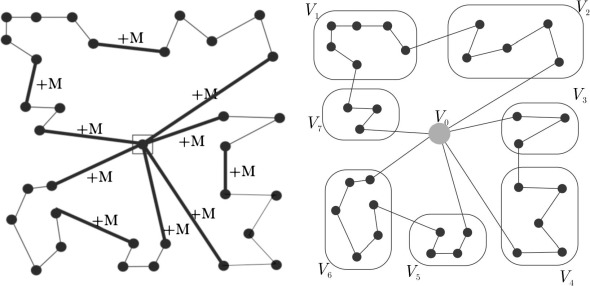
\includegraphics[width=\textwidth,keepaspectratio]{Images/vrp_cluster.jpg}
    \label{fig:clustered_vrp}
    \caption{Left: unclustered VRP with many nodes. Right: clustered subtours by distance}
\end{figure}


By employing a KD tree with ANN search, the algorithm can rapidly identify nearby nodes, significantly reducing the time required to build neighborhoods. This is especially important when the amount of nodes in the problem increases. Traditional brute-force methods such as comparing distances between all nodes, would result in a quadratic time complexity when building the neighborhoods. However, the KD tree structure allows for a more intelligent search of the partitioned space, reducing the time complexity to logarithmic or sub-logarithmic levels.

This acceleration in identifying nearby nodes becomes particularly beneficial when constructing neighborhoods in the VRP/TSP. Efficiently grouping nodes that are close to each other helps us to create neighborhoods of locations that can be served together in a route. This process aids in optimizing the overall travel distance by reducing computational requirements when building the smaller subsets of problems. This method would also allow each neighborhood to be optimized in parallel, since one neighborhood's route doesn't impact any other. Splitting up a large combinatorial optimization problem into smaller, easily parallelizable problems can result in being able to much more thoroughly search the solution space without sacrificing feasible computation time. The combination of KD trees and Approximate Nearest Neighbor search in the context of VRP or TSP could provide us with a powerful tool to quickly identify and group nodes into neighborhoods, thereby enhancing the efficiency of route planning and contributing to the optimization of vehicle routes.

    \printbibliography

\end{document}
